
%(BEGIN_QUESTION)
% Copyright 2012, Tony R. Kuphaldt, released under the Creative Commons Attribution License (v 1.0)
% This means you may do almost anything with this work of mine, so long as you give me proper credit

Sketch all necessary wires and tubes to form a complete working control loop, using the components shown in this diagram:

$$\includegraphics[width=15.5cm]{i01175x01.eps}$$

Also, identify each component in the circuit as being either an electrical {\it source} or an electrical {\it load}, and also show all directions of electric current in the 4-20 mA circuits using conventional flow notation.

\vskip 20pt \vbox{\hrule \hbox{\strut \vrule{} {\bf Suggestions for Socratic discussion} \vrule} \hrule}

\begin{itemize}
\item{} A problem-solving technique useful for making proper connections in pictorial circuit diagrams is to first identify the directions of all DC currents entering and exiting component terminals, as well as the respective voltage polarity marks (+,$-$) for those terminals, based on your knowledge of each component acting either as an electrical {\it source} or an electrical {\it load}.  Discuss and compare how these arrows and polarity marks simplify the task of properly connecting wires between components. 
\end{itemize}

\underbar{file i01175}
%(END_QUESTION)





%(BEGIN_ANSWER)

A very common misconception is that a loop-powered transmitter will function when connected to the Honeywell controller as such:

$$\includegraphics[width=15.5cm]{i01175x04.eps}$$

This is an example of how basic DC circuit analysis (identifying sources, loads, and marking voltage polaritied and current directions) is extremely helpful.  Terminals 8 and 7 on the controller are marked ``1-5 volt PV input'' which tells us the controller's input is expecting a DC voltage between 1 and 5 volts, which the controller will read as though it were a voltmeter.  Thus, the controller (terminals 8 and 7) must be regarded as a load (voltmeter) and not a source of power for the loop-powered transmitter.  Since the loop-powered transmitter is also a load, we see immediately that we have a problem: {\it there is no electrical power source in this circuit!}

Somehow, the circuit must include a DC power supply to provide energy to the transmitter so it may function.  The circuit must also include some provision for converting the 4-20 mA {\it current} signal into a 1-5 V {\it voltage} signal that the controller can measure through terminals 8 and 7.  This means we'll need a 250 $\Omega$ resistor somewhere in the circuit, with the controller connected in parallel with that resistor to measure its 1-5 volt drop.
 
%(END_ANSWER)





%(BEGIN_NOTES)

Only the 24 VDC power supply and the Honeywell controller output are sources.  All other components in the 4-20 mA loop circuits are loads:

$$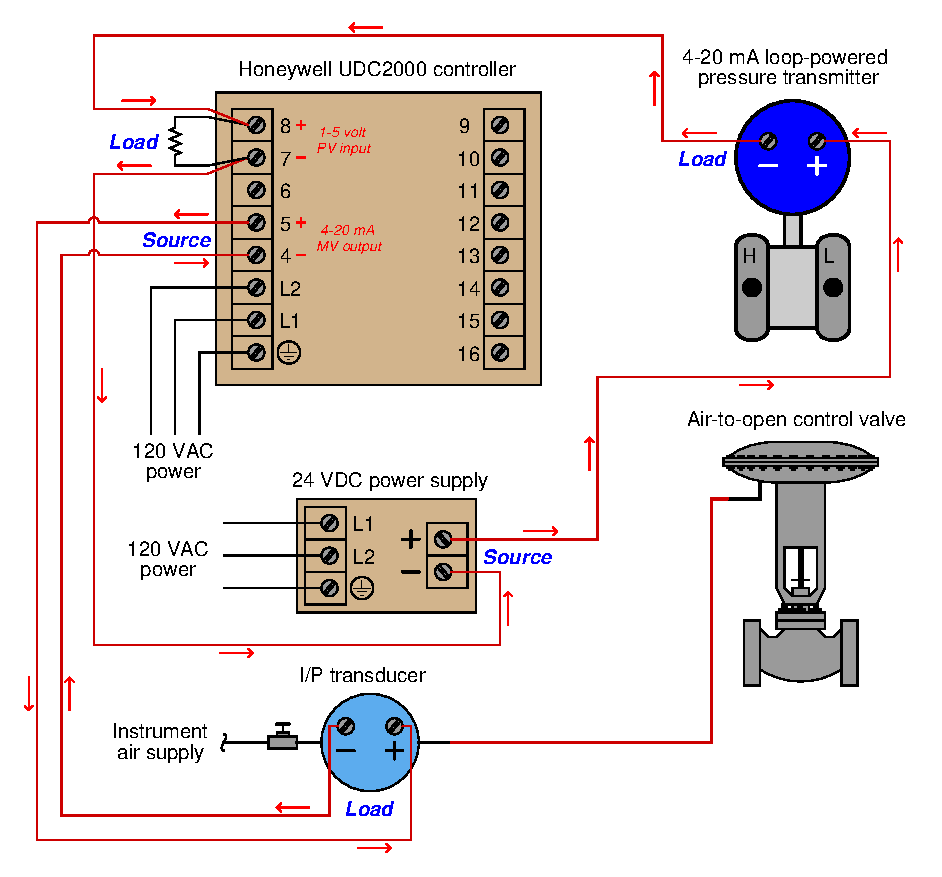
\includegraphics[width=15.5cm]{i01175x02.eps}$$








\vfil \eject

\noindent
{\bf Summary Quiz:}

Sketch the proper wire connections to connect the loop-powered transmitter to the controller PV input:

$$\includegraphics[width=15.5cm]{i01175x03.eps}$$

%INDEX% Pictorial circuit review (4-20 mA loop)

%(END_NOTES)


